\subsection{M.PC.MS - Metriche Soddisfatte}

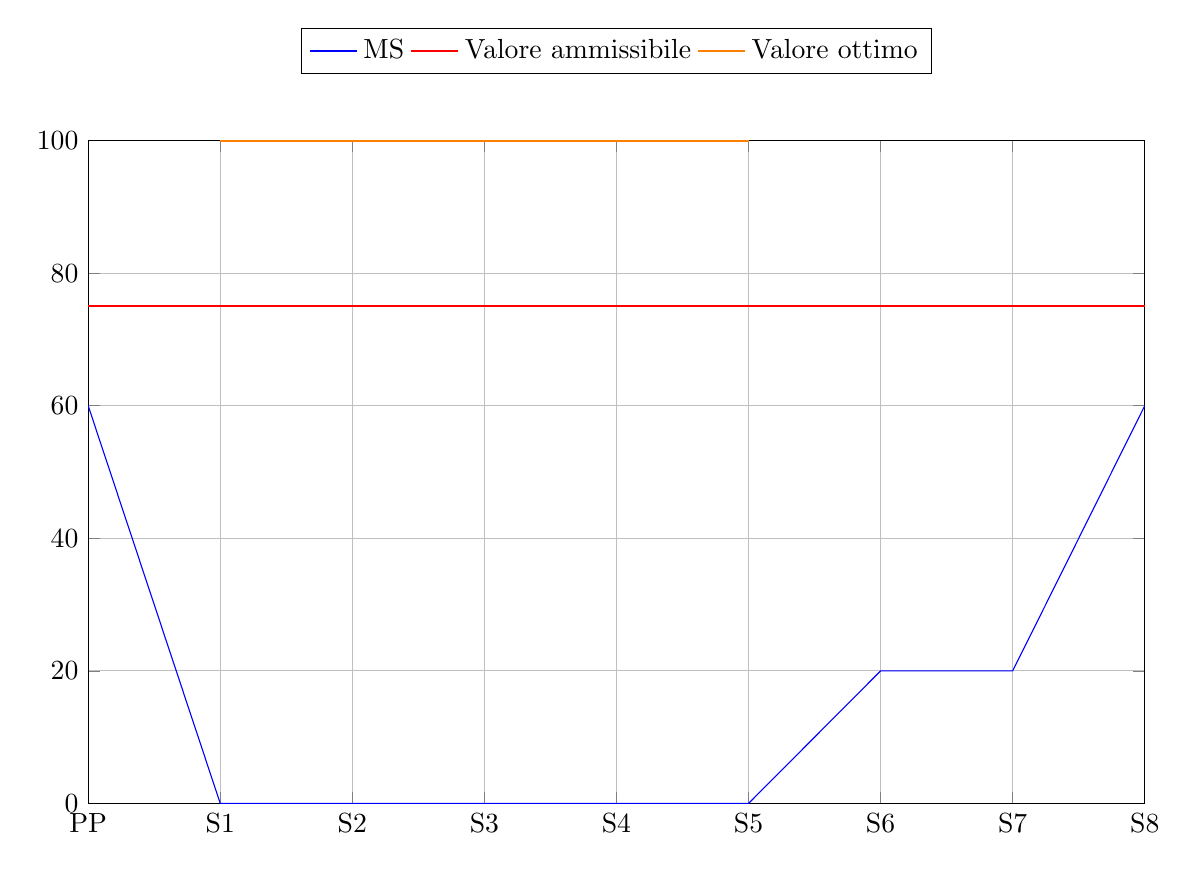
\begin{tikzpicture}
    \begin{axis}[
        width=15cm, height=10cm,
        ymin=0, ymax=100,
        xmin=0, xmax=8,
        xtick={0, 1, 2, 3, 4, 5, 6, 7, 8},
        xticklabels={ PP, S1, S2, S3, S4, S5, S6, S7, S8},
        xlabel={},
        ylabel={},
        grid=major,
        scaled ticks=false,
        legend style={at={(0.5,1.1)}, anchor=south, legend columns=-1},
    ]
    \addplot[color=blue] coordinates {(0, 60) (1, 0) (2, 0) (3, 0) (4, 0) (5, 0) (6, 20) (7, 20) (8, 60)};
    \addlegendentry{MS}
    \addplot[red, thick] coordinates {(0, 75) (8, 75)};
    \addlegendentry{Valore ammissibile}
    \addplot[orange, thick] coordinates {(1, 100) (5, 100)};
    \addlegendentry{Valore ottimo}
    \end{axis}
\end{tikzpicture}
\subsubsection{RTB}
Non è stata assicurata la qualità che si voleva raggiungere per la realizzazione del progetto, i valori inferiori al valore ammissibile sono dovuti
dalle \glossario{metriche} di \glossario{Schedule Variance}, \glossario{Cost Variance}, Correttezza ortografica e Variazione del Piano che non hanno mai raggiunto il valore ammissibile durante lo svolgimento del progetto 
indicando una metodologia di lavoro che non è migliorata sufficientemente con il passare del tempo.